\documentclass[11pt,a4paper]{article}

\usepackage{geometry} \geometry{left=2.2cm, right=2.2cm, top=2.2cm, bottom=2cm}
\parskip 0.15cm 
\setlength{\parindent}{0cm} 
\usepackage{pdflscape}
\usepackage[document]{ragged2e}

\usepackage[T1]{fontenc}  % Set font

\usepackage{lineno}  % Line numbers

\usepackage{amssymb}  % Symbols

\linespread{1.25}  % Linespacing

\usepackage{xcolor} \newcommand{\todo}[1]{\textcolor{red}{\textbf{#1}}}   %

% Tables
\usepackage{multirow} \setlength{\tabcolsep}{4pt}

% Image handling
\usepackage{graphicx} 

\makeatletter \g@addto@macro\@floatboxreset\centering  
\makeatother

\graphicspath{ {img/} }  % Define image path

\usepackage{subfig}  % Compound figures

\usepackage{float}  % Precise figure location

% Bibliography management
\usepackage[style=authoryear, natbib=true, backend=biber]{biblatex}
\addbibresource{lidar.bib}

% Links within document, nice figure formatting
\usepackage[breaklinks]{hyperref} \definecolor{links}{RGB}{0,0,0} \hypersetup{
	breaklinks, colorlinks=true, linkcolor=links, anchorcolor=links,
	citecolor=links, filecolor=links, menucolor=links, runcolor=links,
	urlcolor=links, pdfauthor={John L. Godlee} }
	\def\subsectionautorefname{section} \def\subsubsectionautorefname{section}

\newcommand{\beginsupplement}{% 
	\setcounter{table}{0}
	\renewcommand{\thetable}{S\arabic{table}}% 
	\setcounter{figure}{0}
	\renewcommand{\thefigure}{S\arabic{figure}}% 
}
     
% Variables
\newcommand{\titletext}{Terrestrial LiDAR processing workflow}

% Body
\begin{document}

{\Large{Title: \titletext{}}}

\section{Introduction}

This document details the processing workflow for the terrestrial LiDAR data collected during fieldwork in Bicuar National Park, Angola, and Kilwa District, Tanzania, with the aim of documenting a reproducible workflow.

The project aimed to 

\section{Field methods}

\begin{figure}[H]
\centering
	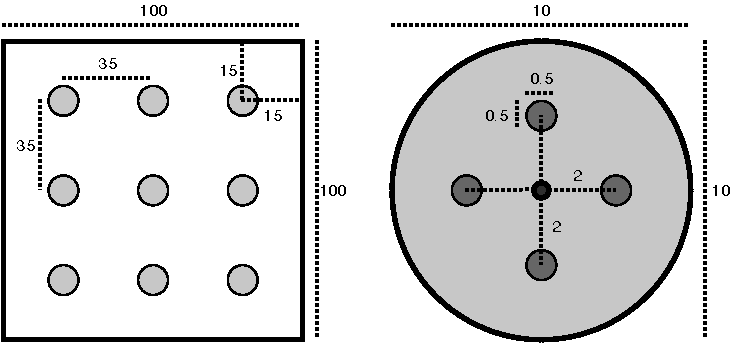
\includegraphics[width=\textwidth]{subplot}
	\caption{The layout of 10 m diameter subplots with each larger 1 ha square plot. Each subplot is situated inside a 15 m buffer from the plot edge, with 35 m between subplot centres. Subplots are arranged in a 3x3 grid. Disc-pasture measurements and biomass samples are located in cardinal directions 2 m from the centre of the subplot. All distances are in metres.}
	\label{subplot}
\end{figure}

\section{Registration}

Scan registration was conducted in Leica Cyclone version XXXX. Targets from each scan were aligned using Cyclone's automatic target acquisition software. 

\section{Voxelization}

The .laz files were voxelised to different voxel sizes depending on the application of the data. For grassy biomass estimation, I used XXX cm\textsuperscript{3} square voxels, while for subplot height profile estimation I used XXX cm\textsuperscript{3} voxels. The reason for this variation in voxel size is ...

\section{Noise reduction}

I used PDAL's XXX noise reduction filter, which ...

\section{Canopy height profiles}

\section{Canopy gap fraction}

\section{Grassy biomass estimation}

\section{Canopy rugosity}

\printbibliography

\end{document}

